\section{$(t, x, z)$空间内的有限差分}
\label{sec:2.7}

如果不是大多数,至少也是很多生产性的偏移处理工作都是在$(t,x,z)$空间内完
成的。为避免被这种三维空间的复杂性所纠缠,我们将首先考虑一下固定$k_x$时在$(z,t)$二
维空间内的偏移。

\subsection{$(z,t)$空间内的偏移}
\label{sec:2.7.1}

可以在$(z',t')$空间内按下列包含有上行波$U$的表格来考察偏移与数据合成的处理过程。
\begin{figure}[H]
\centering
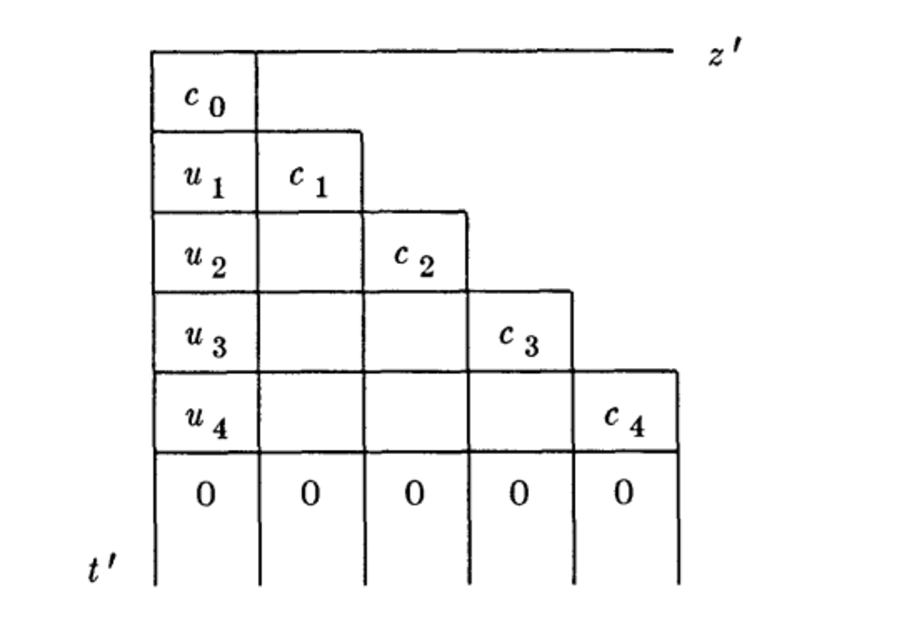
\includegraphics[width=0.65\textwidth]{new/fig-2-7-1}
\caption{差分表}
\label{fig:new/fig-2-7-1}
\end{figure}
在这个表中,在地面$z'=0$所观测到的上行波以$u_t$表示;以$c_t$表示的偏移剖而则沿对角线显
示,因为时间$t=0$时的爆炸反射面的成像条件是在延迟空间内用下式表示的
\begin{subequations}
\begin{equation}
z'=z
\label{eq:ex2.7.2a}
\end{equation}
\begin{equation}
t'=t+z/v
\label{eq:ex2.7.2b}
\end{equation}
\label{eq:ex2.7.2}
\end{subequations}
\begin{equation}
0=t=t'-z'/v
\label{eq:ex2.7.3}
\end{equation}
有最佳聚焦作用的偏移结果并不需要全落在表中所示的45°线上,它可以位于任何直线
上或曲线上,这主要决定于地层的速度。这种曲线构成了速度测定方法的基础(见\ref{sec:3.5}
节), 而在频率域内你就不可能按这种方式来确定速度。

根据\ref{sec:2.1}节的结论,延迟坐标$(t',x',z')$内的上行波$U$的方程为
\begin{equation}
\frac{\partial^2 U}{\partial z'\partial t'}=-\frac{v}{2}\frac{\partial^2 U}{\partial (x')^2}
\label{eq:ex2.7.4}
\end{equation}
然后,对$x$轴迸行Fourier变换,这要假设$v$是$x$的恒定函数,而且假设$U$对$x$的依从关系是正
弦塑函数$\exp(ik_xx)$,因而
\begin{equation}
0=(\frac{v}{2}k_x^2-\frac{\partial^2 }{\partial z'\partial t'})U
\label{eq:ex2.7.5}
\end{equation}
现在,要把这个偏微分方程按广与进行离散化,将要采用矩阵符号,不过'并不是属
于矩阵代数的符号,而是指置于\ref{fig:new/fig-2-7-1}所示表之$(t',z')$平面上的差分系数组成的矩
阵。令符号$*$来代表$(z,t)$空间内的褶积运算,相继求导数实际是一种褶积过程,所以
$\partial/\partial z \partial/\partial t=\partial^2/(\partial z\partial t)$这种概念用下式表示:
\begin{equation}
\begin{bmatrix}
-1 & +1
\end{bmatrix}
*
\begin{bmatrix}
-1 \\
1
\end{bmatrix}
=
\begin{bmatrix}
1&-1\\
-1&1
\end{bmatrix}
\label{eq:ex2.7.6}
\end{equation}
所以,式\ref{eq:ex2.7.5}的差分形式为
\begin{equation}
0=\{\frac{v}{2}\frac{\Delta z'\Delta t'}{4}k_x^2
\begin{bmatrix}
1&1\\
1&1
\end{bmatrix}
-
\begin{bmatrix}
1&-1\\
-1&1
\end{bmatrix}
\}*U
\label{eq:ex2.7.7}
\end{equation}
其中出现$1/4$是因为要在网格的四个位置上取$U$的平均。

两个算子之和按下列形式恒有$\mid b \mid \geq \mid s \mid $
\begin{equation}
0 =
\begin{bmatrix}
s&b\\
b&s
\end{bmatrix}
*U
\label{eq:ex2.7.8}
\end{equation}
现在将利用式\ref{eq:ex2.7.8}中的差分系数以各$U$值来填满\ref{fig:new/fig-2-7-1}所示的表。

已知三个方格中的$U$值,则可根据下面隐含的两种运算中的一种
\begin{figure}[H]
\centering
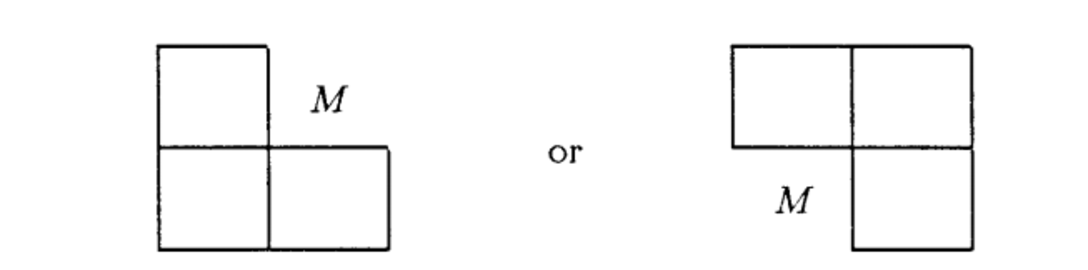
\includegraphics[width=0.65\textwidth]{new/fig-2-7-2}
\caption{左边a,右边b}
\label{fig:new/fig-2-7-2}
\end{figure}

就能够决定缺失的一个值$M$。可证明,由于$\mid b \mid \geq \mid s \mid $,按下面的格式进行$M$值的计算是不稳
定的:
\begin{figure}[H]
\centering
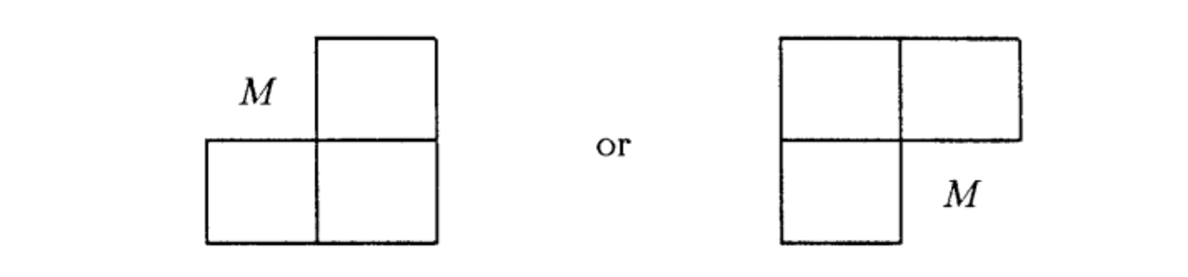
\includegraphics[width=0.65\textwidth]{new/fig-2-7-3}
\caption{左边a,右边b}
\label{fig:new/fig-2-7-3}
\end{figure}
很显然,如果$s$等于零,就会存在用零来除的问题。根据稳定性分析毫无困难就可证明,式
\ref{fig:new/fig-2-7-3}的运算方式会引起微小扰动呈指数增长。

有一个值得作一作的练习:在零倾角假设$(k_x=0)$下,用式\ref{eq:ex2.7.8}的算子中的数值
去填满\ref{fig:new/fig-2-7-1}所示表中的各元素.将会发现,$u_t$值沿$z$方向横向移动通过该表而无变化,
正如由该表所能预料到的,这意味着$c_t=u_t$。沿$z$方向有缓慢变化,就是提醒我们,沿$z$轴的
采样已经过密了。实际上,沿$z$轴迸行少量点的采样要比通常沿$t$轴进行采样节省很多计算时
间。

\subsection{$(t,x,z)$空间的15度绕射程序}
\label{sec:2.7.2}

要理解$(t,x,z)$空间内的$15$度偏移,最容易的办法就是考虑$(z,t)$空间的偏移。
现在,我们不采用标量函数$U(k_x)$,而是利用一个向量$\mathbf{u}$,这个向量的各分量$u_j$是在
$x=j\Delta x$点上测定的压力。把$k_x^2$看作是一种三对角线矩阵,称作$\mathbf{T}$,其主对角线上为$(-1,
2,-1)$。注意,$k_x^2$恒为正值,故而$\mathbf{T}$是一个其主对角线上均为正值元素的正定矩阵。采用
\ref{eq:ex2.7.7}并以$\alpha$表示左侧常数,则
\begin{equation}
0 = \{
\alpha\mathbf{T}
\begin{bmatrix}
\mathbf{I}&\mathbf{I}\\
\mathbf{I}&\mathbf{I}
\end{bmatrix}
-
\begin{bmatrix}
\mathbf{I}&-\mathbf{I}\\
-\mathbf{I}&\mathbf{I}
\end{bmatrix}
\}*\mathbf{u}
=
\begin{bmatrix}
\alpha\mathbf{T}-\mathbf{I}&\alpha\mathbf{T}+\mathbf{I}\\
\alpha\mathbf{T}+\mathbf{I}&\alpha\mathbf{T}-\mathbf{I}
\end{bmatrix}*\mathbf{u}
\label{eq:ex2.7.11}
\end{equation}
现在考虑一种模拟程序。利用\ref{fig:new/fig-2-7-2}所示格式的差分系数表,开始向下进入地层内
部进行计算,对未知数求解式\ref{eq:ex2.7.11},并略去所有撇号,得
\begin{equation}
(\alpha\mathbf{T}+\mathbf{I})
\mathbf{u}_{t+1,z}=
-[
(\alpha\mathbf{T}+\mathbf{I})
\mathbf{u}_{t,z+1}+
(\alpha\mathbf{T}-\mathbf{I})
(\mathbf{u}_{t,z}+\mathbf{u}_{t+1,z+1})
]
\label{eq:ex2.7.12}
\end{equation}
首先,求出右端表达式的值,左端是有关待求的未知数$\mathbf{u}_{t+1,z}$的三对角线方程组。容许应用
于式\ref{eq:ex2.7.12}的序列受\ref{fig:new/fig-2-7-2}所示差分系数表所支配。

留意一下先前关于具有中等倾角之波场的评论,即对$z'$轴进行采样无需像$t'$轴那样稠
密。我们可沿$z'$方向交错跳跃地进行计算。在程序\ref{lst:code2.7.1}所示计算机程序中,所选择的具体计算顺序由下表所列数字表示:
\begin{figure}[H]
\centering
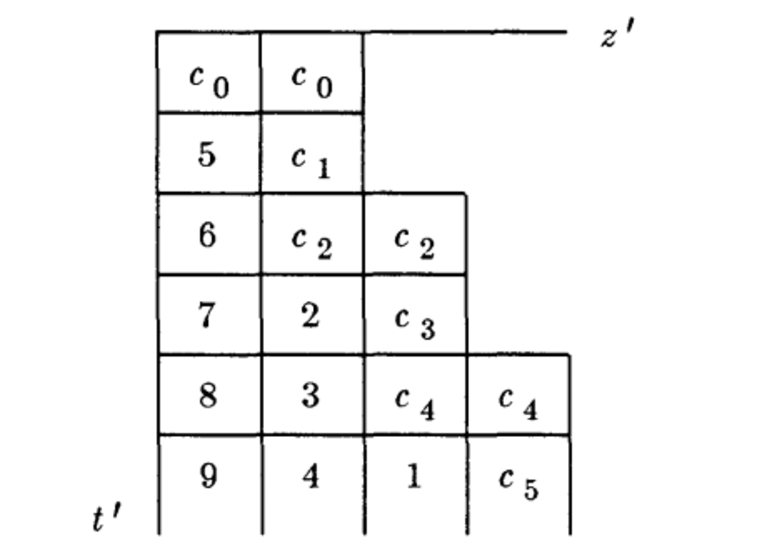
\includegraphics[width=0.65\textwidth]{new/fig-2-7-4}
\caption{程序\ref{lst:code2.7.1}所示的差分系数表}
\label{fig:new/fig-2-7-4}
\end{figure}
\begin{listing}[H]
    \caption{时间域绕射程序(Clayton,Gonzalez,
JFC,Hale)}
    \inputminted{Fortran}{code2-7-1.f90}
    \label{lst:code2.7.1}
\end{listing}
在$t'$空间的点数不是严格等于$z'$空间的点数时,表中所示有一个逃
避不了的实际问题,那就是必须沿网格上的一个对角线进行内插才能得
出地层影像。表格\ref{fig:new/fig-2-7-4}中的粗略内插是为了说明波场沿$t'$方向快
速变化而沿$z'$方同缓慢变化这种假设,即小倾角假设。

图\ref{fig:txz/diffr}所示是由检验程序所产生的活动电影内之最后画面。习题
1提出对程序\ref{lst:code2.7.1}作一些次要的改变,就能使它由绕射程序转换
为偏移程序。修改后,该程序实质上就是Johnson与Claerbout(1971)及Doherty与Claerbout(1972)
所引进的原始波动方程偏移程序了。
\begin{figure}[H]
\centering
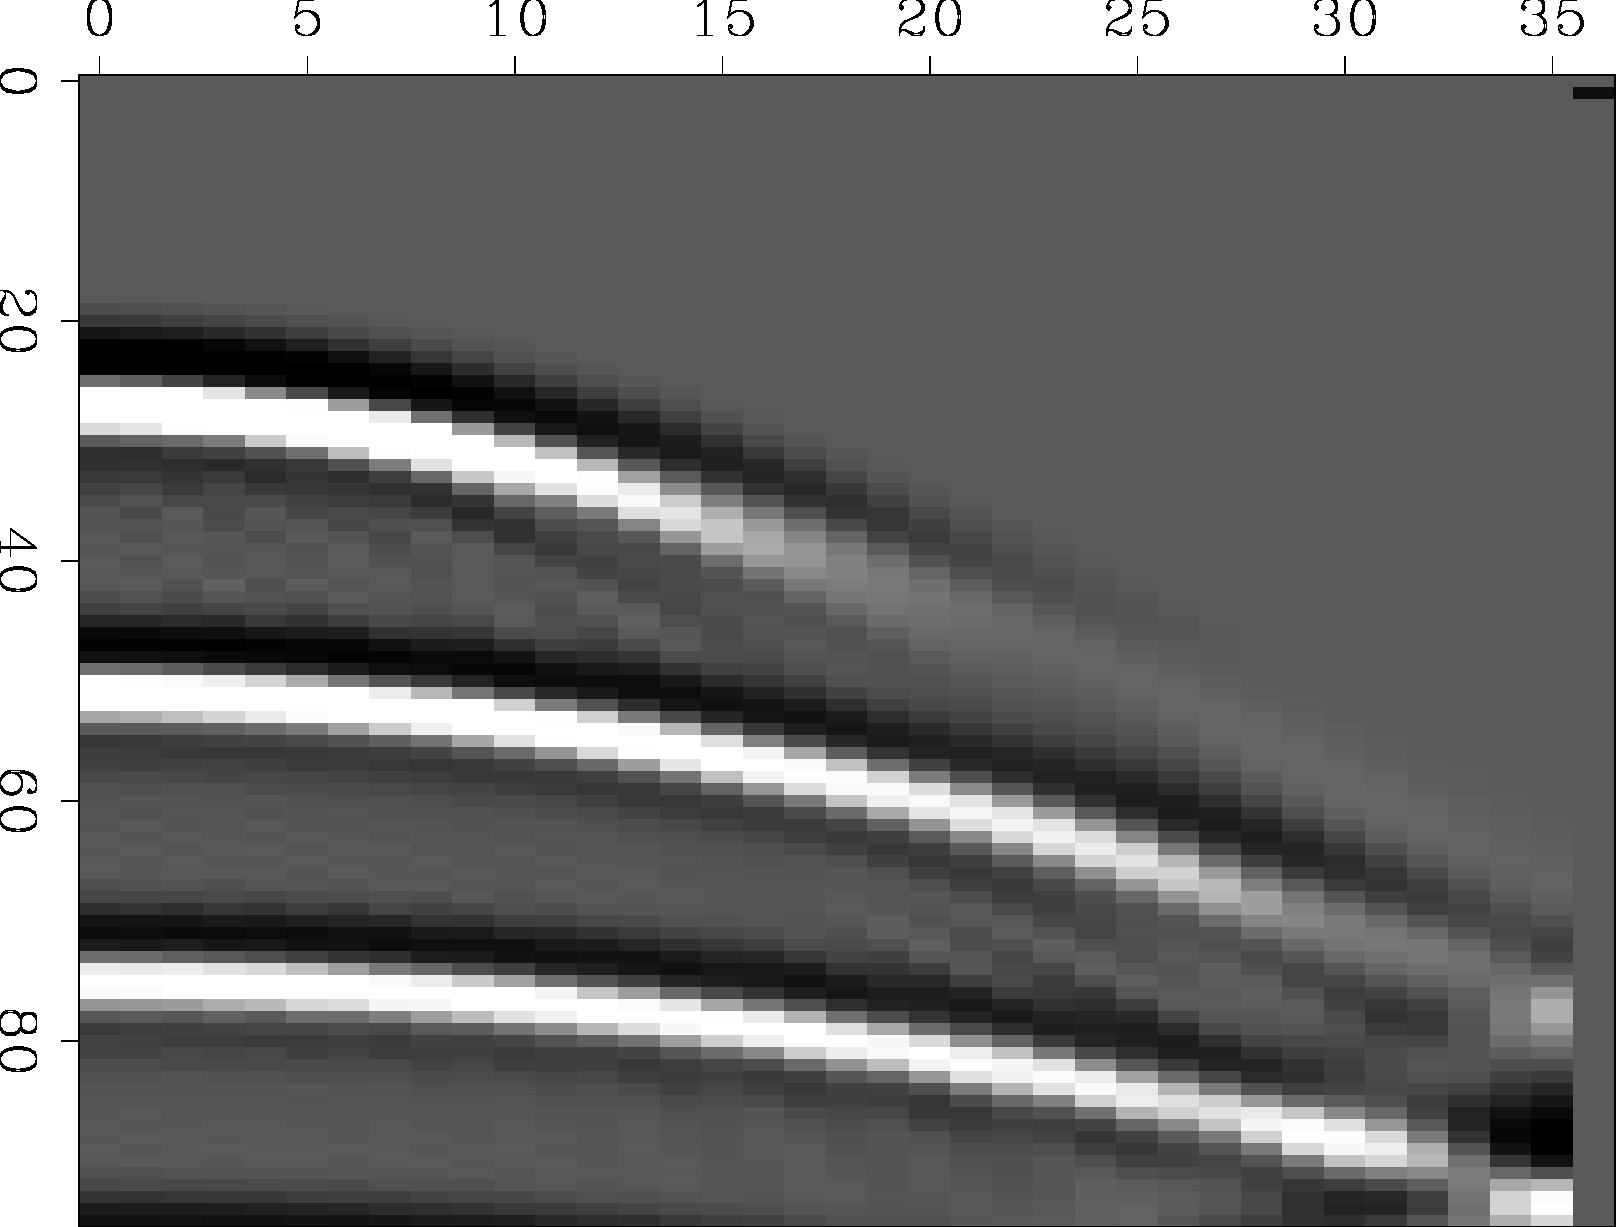
\includegraphics[width=0.65\textwidth]{txz/diffr}
\caption[diffr]{向下延拓活动电影最后画面内的绕射}
\label{fig:txz/diffr}
\end{figure}

\subsection{不可在时间域内进行时移}
\label{sec:2.7.3}

你也许希望在具有横向速度变化的$(x,z,t)$空间中作偏移,这
时,完成薄透镜项这一步骤要采用时移的办法,而不是乘以
$\exp\{i\omega[\frac{1}{v(x,z)}-\frac{1}{\bar{v}(z)}]\}$。在需要按整数雜单位对数据进行
时移时,完成时移是一件轻而易举的事。可是,按数宇采样单位的非整数分数来成批进行时
移,那就像恶梦般地可怕了。这时,要求用多点内插算子,即使这样,脉冲还是有弥散的趋
势。因此,把透镜项留在频率域内去处理,大概是最好的办法了。

\subsection{$(t,x,z)$空间内的45度方程}
\label{sec:2.7.4}

45°偏移比15°偏移稍为困难一些,因为时间域内的算子这时姑较高阶的算子,但是方法
还是类似于15°方程和递归倾角滤波的那些方法。直接的处理办法只需记下差分系数表即
可,我过去作这类工作时曾发现,最容易的办法是利用$Z$变换,这时用双线变换$\frac{1}{2}(\frac{1+z}{1-z})$来
代表$1/(-i\omega\Delta t)$。有许多种途径可使代数运算不太繁琐,一种途径是把所有含$Z$的项均化
至分子内,然后将$z$的同幂项集中起来,另一种称作积分法的途径是使$1/(1-Z)$保持为若干项。凡包括$1/(1-Z)$
的项在计算机中均用这样的缓冲区代表:这种缓冲区含有双无限大时
间至时间$t$的和。变换方法在\ref{sec:4.6}节内讨论,它的真正好处就是它使稳定性分析更为系统化。

\subsection{习 题}
\label{sec:2.7.5}

\begin{enumerate}
\item 修改程序\ref{lst:code2.7.1},使之成为偏移程序。脉冲函数输入应变成近似半圆。
\item 对程序\ref{lst:code2.7.1}进行重要改变,使之变成一种低通倾角滤波程序。
\item 试考虑$(z,t,k_x)$空间中的45°偏移程序.求出6点差分系数表内的各系数。
  其中,三个点属于时间,两个点属于深度。为简单起见,取$v=1$,$\Delta t=1$
  及$\Delta z=1$。设用$\mathbf{T}$代
  替$k_x^2$就可将这种分析交换至$x$域$(\Delta x=1)$。这时将必须求解什么三对角线方程组?
\end{enumerate}

